\section{Diseño de los autómatas}

Los autómatas de las Figuras~\ref{fig:identificadores}, \ref{fig:numeros} y \ref{fig:operadores} representan las categorías con mayor posibilidad de superposición. La flecha de entrada identifica el estado inicial $q_0$ y la doble circunferencia identifica los estados aceptadores, con la categoría indicada en su interior. Las transiciones omitidas llevan a un estado muerto implícito. Al tokenizar, se conserva la última aceptación y se devuelve el prefijo aceptado más largo; el carácter que inicia el siguiente token queda sin consumir. La validación de fronteras numéricas puede sustituir ese prefijo por un diagnóstico, según la especificación anterior.

\begin{figure}[H]
  \centering
  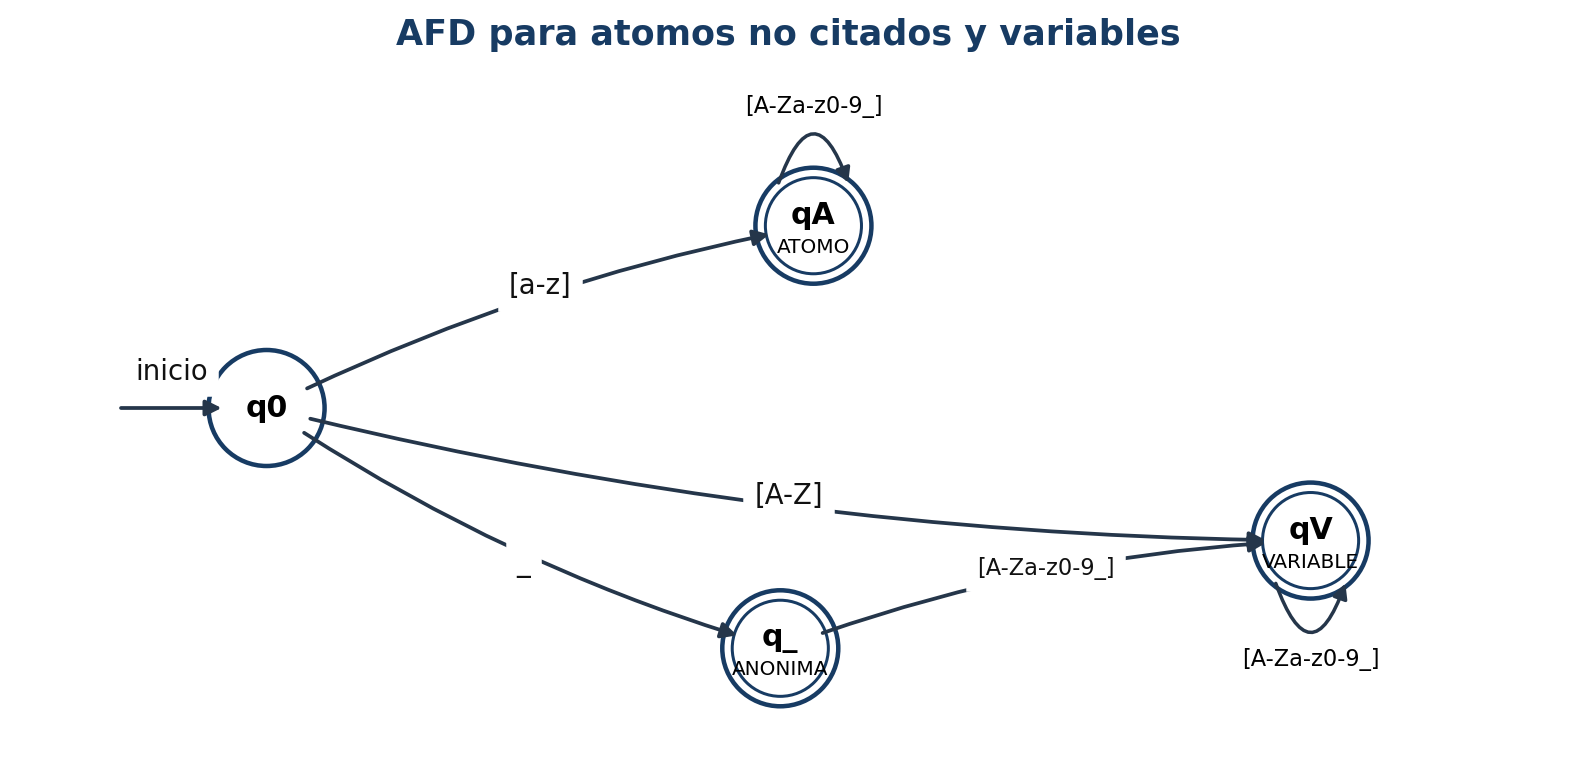
\includegraphics[width=0.98\textwidth]{figuras/afd_identificadores.png}
  \caption{AFD para identificadores. El estado $q_A$ requiere reclasificar \texttt{is} y \texttt{mod}.}
  \label{fig:identificadores}
\end{figure}

\begin{figure}[H]
  \centering
  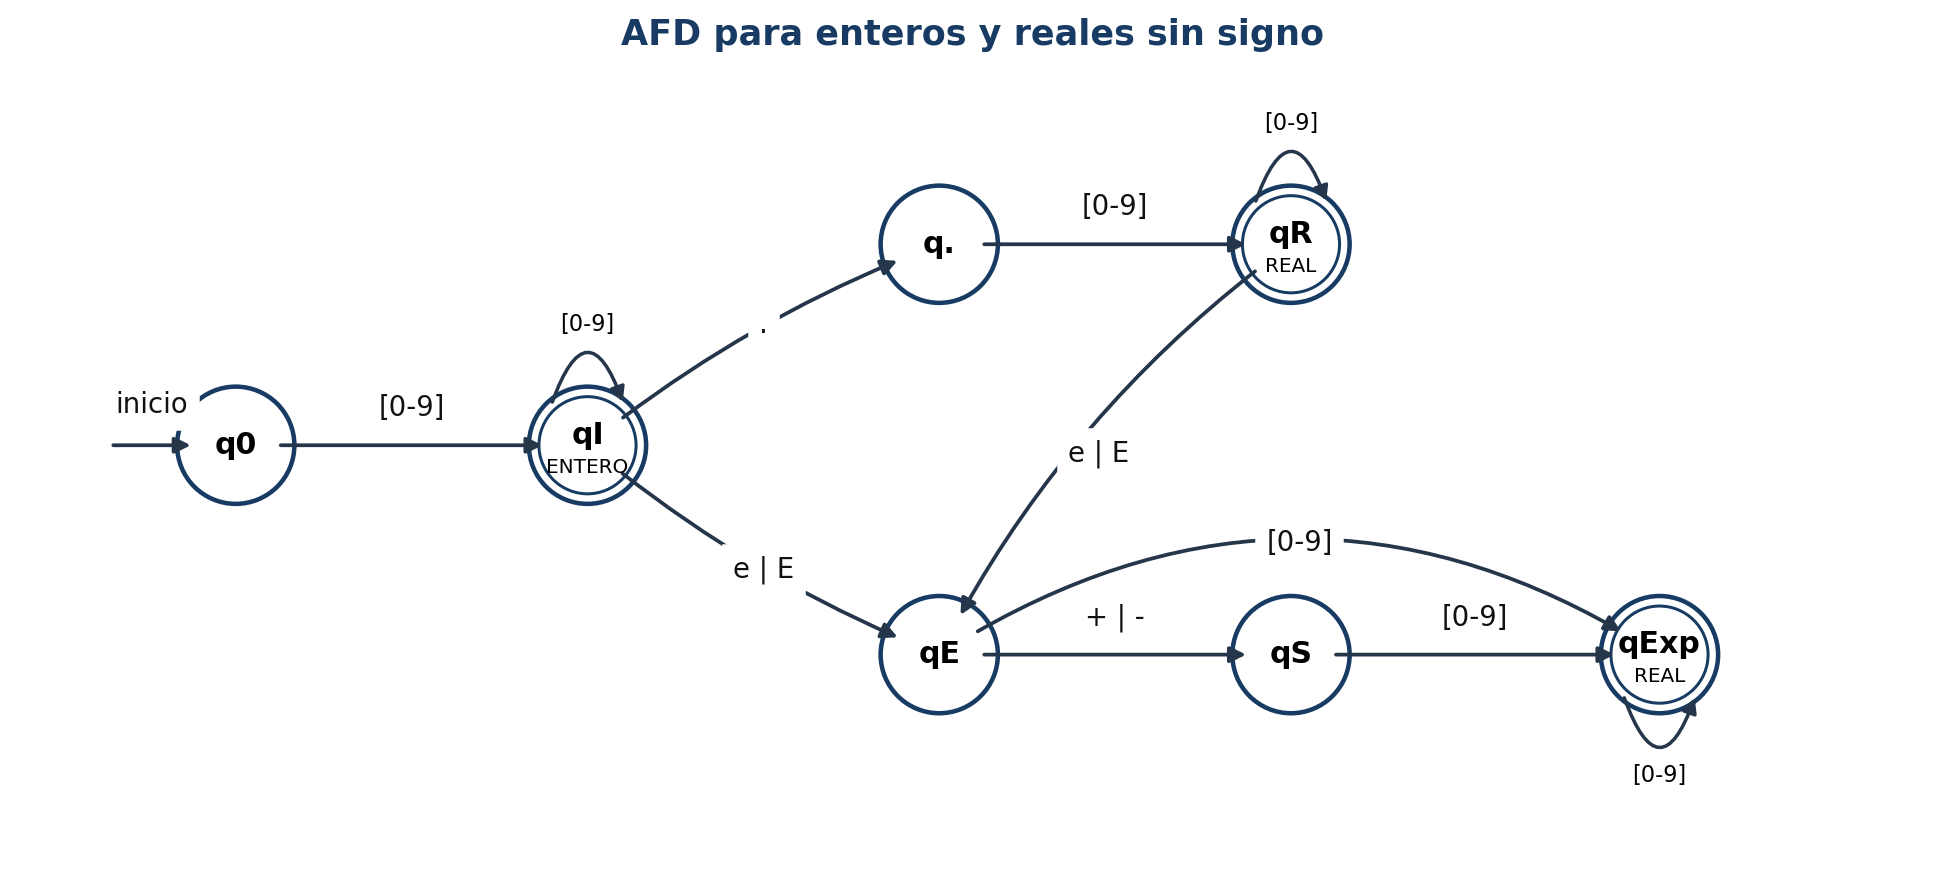
\includegraphics[width=0.98\textwidth]{figuras/afd_numeros.png}
  \caption{AFD para enteros y reales sin signo léxico.}
  \label{fig:numeros}
\end{figure}

\begin{figure}[H]
  \centering
  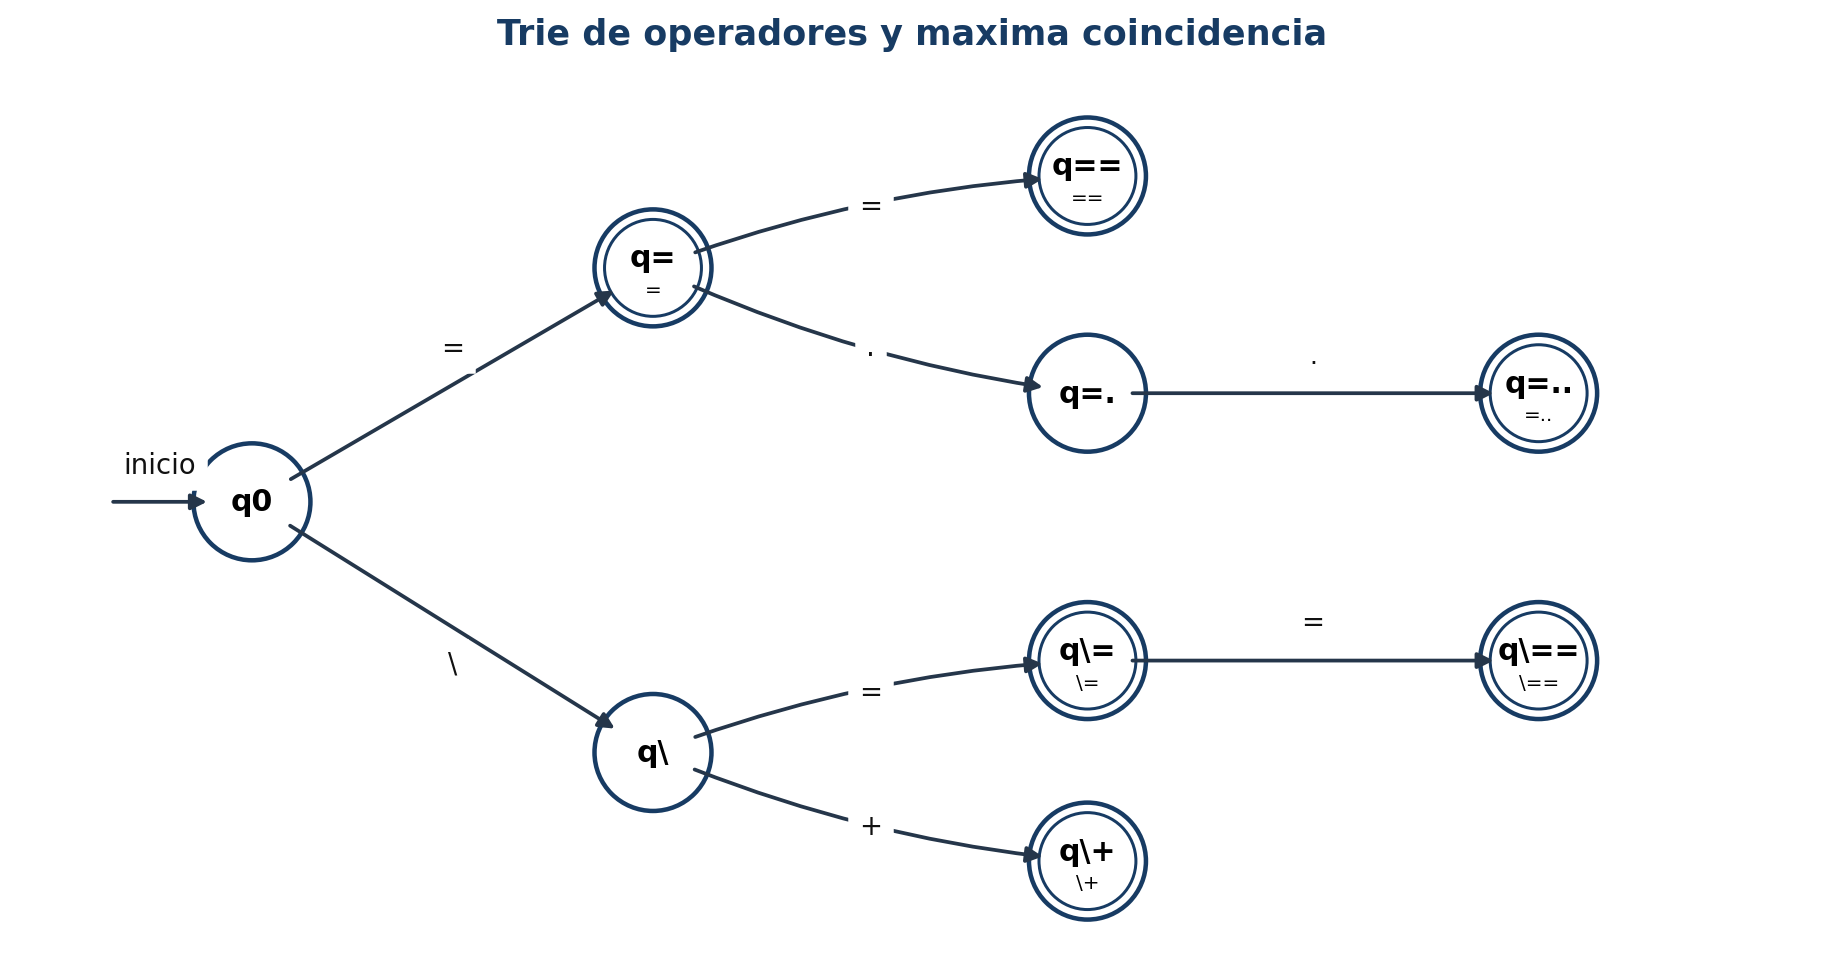
\includegraphics[width=0.98\textwidth]{figuras/afd_operadores.png}
  \caption{Fragmento del trie de operadores con prefijos compartidos.}
  \label{fig:operadores}
\end{figure}

El estado $q_{\_}$ acepta únicamente la variable anónima. Si se lee otro carácter de $C$, se pasa a $q_V$ y el lexema completo es una variable con nombre. En el autómata numérico, $q_I$, $q_R$ y $q_{Exp}$ aceptan ENTERO, REAL y REAL, respectivamente; $q_{.}$, $q_E$ y $q_S$ no aceptan. Por ejemplo, \texttt{2e-3} recorre $q_0,q_I,q_E,q_S,q_{Exp}$. Para \texttt{12.}, la última aceptación es $q_I$: el punto queda como delimitador. Para \texttt{1e+}, la frontera detecta un exponente incompleto y produce un error, en lugar de emitir el entero \texttt{1}.

El trie mostrado es un fragmento: \texttt{=} y \verb|\=| ya aceptan, pero pueden prolongarse hasta \texttt{==}, \texttt{=..} y \verb|\==|. En el lexer, la tupla completa \texttt{SYMBOL\_OPERATORS}, ordenada por longitud descendente, representa las demás ramas. Un delimitador requiere una transición desde el inicio a su estado aceptador; espacios y comentarios terminados alcanzan estados de descarte.

\subsection{Autómatas para citas y comentarios}

Un mismo AFD sirve para ATOMO\_CITADO y CADENA parametrizando la comilla $c$ (simple o doble). Sea $E=\{n,t,r,\backslash,\text{comilla simple},\text{comilla doble}\}$ el conjunto permitido después de una barra. La Tabla~\ref{tab:afd-citas} especifica todas las transiciones que no van al estado muerto. $Q_0$ es inicial y $Q_F$ es el único aceptador: emite el tipo determinado por $c$. Las clases de cada fila son disjuntas; en $Q_I$ la comilla opuesta es un carácter ordinario.

\begin{table}[H]
\centering
\small
\caption{AFD parametrizado para átomos citados y cadenas.}
\label{tab:afd-citas}
\begin{tabularx}{\textwidth}{C{1.5cm}Y C{1.5cm} L{4.0cm}}
\toprule
\tableheader{Origen} & \tableheader{Entrada} & \tableheader{Destino} & \tableheader{Interpretación} \\
\midrule
$Q_0$ & $c$ & $Q_I$ & Apertura \\
\rowcolor{palegray} $Q_I$ & $\Sigma\setminus\{c,\backslash,\mathrm{CR},\mathrm{LF}\}$ & $Q_I$ & Contenido ordinario \\
$Q_I$ & $\backslash$ & $Q_E$ & Inicio de escape \\
\rowcolor{palegray} $Q_E$ & $E$ & $Q_I$ & Escape admitido \\
$Q_I$ & $c$ & $Q_F$ & Cierre y aceptación \\
\bottomrule
\end{tabularx}
\end{table}

CR, LF o fin de archivo antes de $Q_F$ generan un diagnóstico de cita sin cierre. Un escape fuera de $E$ impide aceptar el literal; la implementación conserva la primera secuencia inválida y continúa hasta su cierre o fin de línea para recuperar el análisis. Este recorrido de recuperación no convierte el literal erróneo en un token aceptado.

Para comentarios de línea, el estado inicial $L_0$ pasa con \texttt{\%} a $L_1$, que es aceptador y repite con $\Sigma\setminus\{\mathrm{CR},\mathrm{LF}\}$. Al encontrar un salto o fin de archivo se descarta el comentario. El salto queda para el reconocedor de espacios. Para comentarios de bloque, la Tabla~\ref{tab:afd-bloque} reconoce el primer cierre \texttt{*/}; $B_0$ es inicial y $B_F$ es el único aceptador. Un fin de archivo en $B_2$ o $B_3$ produce un error de comentario sin cierre. La entrada \texttt{/*} activa este reconocedor antes que el operador \texttt{/}.

\begin{table}[H]
\centering
\small
\caption{Transiciones no muertas del AFD de comentarios de bloque.}
\label{tab:afd-bloque}
\begin{tabularx}{\textwidth}{C{1.5cm}Y C{1.5cm} L{4.0cm}}
\toprule
\tableheader{Origen} & \tableheader{Entrada} & \tableheader{Destino} & \tableheader{Interpretación} \\
\midrule
$B_0$ & \texttt{/} & $B_1$ & Primer carácter \\
\rowcolor{palegray} $B_1$ & \texttt{*} & $B_2$ & Apertura completa \\
$B_2$ & $\Sigma\setminus\{\texttt{*}\}$ & $B_2$ & Contenido \\
\rowcolor{palegray} $B_2$ & \texttt{*} & $B_3$ & Posible cierre \\
$B_3$ & \texttt{*} & $B_3$ & Mantiene posible cierre \\
\rowcolor{palegray} $B_3$ & $\Sigma\setminus\{\texttt{*},\texttt{/}\}$ & $B_2$ & Continúa contenido \\
$B_3$ & \texttt{/} & $B_F$ & Cierre y descarte \\
\bottomrule
\end{tabularx}
\end{table}

\subsection{Determinización representativa}

Para mostrar la construcción de subconjuntos se utiliza el lenguaje $LC^*$ de identificadores iniciados en minúscula, antes de reclasificar las palabras \texttt{is} y \texttt{mod}. En este ejemplo, la etiqueta ATOMO designa ese patrón estructural. Se parte de un AFN deliberadamente no mínimo que divide la primera letra en dos ramas equivalentes. El estado $q_0$ posee transiciones $\varepsilon$ hacia $p_0$ y $r_0$; desde $p_0$, una letra de $[a\text{-}m]$ lleva a $p_1$, mientras que desde $r_0$ una letra de $[n\text{-}z]$ lleva a $r_1$. Los estados $p_1$ y $r_1$ son aceptadores y repiten con cualquier carácter de $C$. La transformación aplica la construcción de subconjuntos y luego refina particiones para obtener estados equivalentes \cite{hopcroft}.

Formalmente, $Q=\{q_0,p_0,r_0,p_1,r_1\}$, el inicial es $q_0$ y $F=\{p_1,r_1\}$. Las clases de entrada son $[a\text{-}m]$, $[n\text{-}z]$, $U\cup D\cup\{\_\}$ y $\Sigma\setminus C$. Para esta última, todas las transiciones del AFN son vacías; se omite su columna para facilitar la lectura.

\begin{table}[H]
\centering
\small
\caption{Transiciones del AFN representativo.}
\label{tab:afn}
\begin{tabularx}{0.92\textwidth}{C{1.7cm}C{2.1cm}C{2.1cm}C{2.1cm}Y}
\toprule
\tableheader{Estado} & \tableheader{$\varepsilon$} & \tableheader{$[a$--$m]$} & \tableheader{$[n$--$z]$} & \tableheader{$U\cup D\cup\{\_\}$} \\
\midrule
$q_0$ & $\{p_0,r_0\}$ & $\varnothing$ & $\varnothing$ & $\varnothing$ \\
\rowcolor{palegray} $p_0$ & $\varnothing$ & $\{p_1\}$ & $\varnothing$ & $\varnothing$ \\
$r_0$ & $\varnothing$ & $\varnothing$ & $\{r_1\}$ & $\varnothing$ \\
\rowcolor{palegray} $p_1$ & $\varnothing$ & $\{p_1\}$ & $\{p_1\}$ & $\{p_1\}$ \\
$r_1$ & $\varnothing$ & $\{r_1\}$ & $\{r_1\}$ & $\{r_1\}$ \\
\bottomrule
\end{tabularx}
\end{table}

Para un subconjunto $S$ y un carácter $a$ se calcula
\[
\delta_D(S,a)=\operatorname{cl}_{\varepsilon}
\left(\bigcup_{q\in S}\delta_N(q,a)\right).
\]
La clausura-$\varepsilon$ inicial es $D_0=\{q_0,p_0,r_0\}$. Al mover ese conjunto con $[a\text{-}m]$ se obtiene $D_1=\{p_1\}$; con $[n\text{-}z]$ se obtiene $D_2=\{r_1\}$. Cualquier clase sin transición conduce a $D_{\bot}=\varnothing$. Como $p_1$ y $r_1$ repiten con $C$, no aparecen nuevos subconjuntos. Un subconjunto acepta si intersecta $F$, por lo que solo $D_1$ y $D_2$ son aceptadores. Los cuatro estados son alcanzables: con $\varepsilon$, \texttt{a}, \texttt{n} y \texttt{0}, respectivamente.

\begin{table}[H]
\centering
\small
\caption{Tabla de transición obtenida mediante construcción de subconjuntos.}
\label{tab:determinizado}
\begin{tabularx}{\textwidth}{L{3.4cm}C{1.9cm}C{1.9cm}C{3.3cm}Y}
\toprule
\tableheader{Estado AFD} & \tableheader{$[a$--$m]$} & \tableheader{$[n$--$z]$} & \tableheader{$U\cup D\cup\{\_\}$} & \tableheader{Aceptación} \\
\midrule
$D_0=\{q_0,p_0,r_0\}$ & $D_1$ & $D_2$ & $D_{\bot}$ & No \\
\rowcolor{palegray} $D_1=\{p_1\}$ & $D_1$ & $D_1$ & $D_1$ & ATOMO \\
$D_2=\{r_1\}$ & $D_2$ & $D_2$ & $D_2$ & ATOMO \\
\rowcolor{palegray} $D_{\bot}=\varnothing$ & $D_{\bot}$ & $D_{\bot}$ & $D_{\bot}$ & No \\
\bottomrule
\end{tabularx}
\end{table}

Para todo estado de la Tabla~\ref{tab:determinizado}, una entrada de $\Sigma\setminus C$ conduce a $D_{\bot}$. Por ejemplo, \texttt{padre\_1} sigue $D_0,D_2,D_2,D_2,D_2,D_2,D_2,D_2$ y acepta; \texttt{Padre} pasa inmediatamente al estado muerto. No se confunde rechazo como átomo con error global: el despachador reconoce \texttt{Padre} mediante el AFD de variables.

\subsection{Minimización}

La partición inicial es $P_0=\{\{D_1,D_2\},\{D_0,D_{\bot}\}\}$: el primer bloque contiene los estados que aceptan ATOMO y el segundo, los que no aceptan. El bloque no aceptador se divide porque desde $D_0$ una letra minúscula alcanza aceptación, mientras que desde $D_{\bot}$ toda entrada permanece en el estado muerto. En cambio, $D_1$ y $D_2$ no se separan: ambos aceptan exactamente los sufijos de $C^*$ y cualquier carácter fuera de $C$ lleva al mismo estado muerto. La partición estable es $P_1=\{\{D_1,D_2\},\{D_0\},\{D_{\bot}\}\}$, por lo que $D_1$ y $D_2$ se fusionan en la clase de equivalencia $D_A=[D_1]=[D_2]$.

Los tres estados restantes son distinguibles: el sufijo vacío $\varepsilon$ separa $D_A$ de ambos estados no aceptadores, y el sufijo \texttt{a} distingue $D_0$ de $D_{\bot}$. Como todos son alcanzables, el AFD completo de tres estados es mínimo. En los diagramas parciales se omite el estado muerto y quedan dos estados visibles para este patrón. Esta minimización no corresponde al lexer entero: un AFD que emita varias categorías debe conservar las etiquetas de token al formar su partición inicial.

\begin{table}[H]
\centering
\small
\caption{AFD mínimo para el ejemplo representativo.}
\label{tab:minimo}
\begin{tabularx}{\textwidth}{L{3.4cm}C{1.9cm}C{1.9cm}C{3.3cm}Y}
\toprule
\tableheader{Estado mínimo} & \tableheader{$[a$--$m]$} & \tableheader{$[n$--$z]$} & \tableheader{$U\cup D\cup\{\_\}$} & \tableheader{Aceptación} \\
\midrule
$D_0$ & $D_A$ & $D_A$ & $D_{\bot}$ & No \\
\rowcolor{palegray} $D_A=[D_1]=[D_2]$ & $D_A$ & $D_A$ & $D_A$ & ATOMO \\
$D_{\bot}$ & $D_{\bot}$ & $D_{\bot}$ & $D_{\bot}$ & No \\
\bottomrule
\end{tabularx}
\end{table}

Las entradas de $\Sigma\setminus C$ llevan a $D_{\bot}$ también en la Tabla~\ref{tab:minimo}. La reclasificación de \texttt{is} y \texttt{mod} se mantiene después del reconocimiento: fusionar los estados estructurales no elimina la consulta del lexema completo.

\subsection{Estrategia integrada y correspondencia con el código}

\subsubsection{Trazas de aceptación y fronteras}

Las siguientes trazas separan la aceptación del autómata de la decisión del lexer sobre la frontera del lexema. Un estado no aceptador intermedio no implica que toda la entrada sea errónea: puede existir una aceptación anterior. A su vez, la regla numérica de frontera puede impedir emitir ese prefijo si ocultaría un número mal formado.

\begin{table}[H]
\centering
\small
\caption{Trazas representativas y resultado observable.}
\begin{tabularx}{\textwidth}{L{2cm}Y L{5.5cm}}
\toprule
\tableheader{Entrada} & \tableheader{Recorrido relevante} & \tableheader{Resultado del lexer} \\
\midrule
\texttt{12.} & $q_0,q_I,q_I,q_{.}$. La última aceptación está antes del punto. & ENTERO \texttt{12}, PUNTO \texttt{.}. \\
\rowcolor{palegray} \texttt{2e-3} & $q_0,q_I,q_E,q_S,q_{Exp}$. El signo pertenece al exponente. & Un REAL con lexema \texttt{2e-3}. \\
\texttt{1e+} & $q_0,q_I,q_E,q_S$. El estado final no acepta y el sufijo inicia con \texttt{e}. & Un error por \texttt{1e+}; no se emite ENTERO. \\
\rowcolor{palegray} \texttt{3.14.15} & Se alcanza $q_R$ en \texttt{3.14}; la frontera siguiente es punto más dígito. & Un error por todo \texttt{3.14.15}. \\
\texttt{\_X} & $q_0,q_{\_},q_V$. La aceptación de variable prolonga la anónima. & VARIABLE con índice; no se emite \texttt{\_} separado. \\
\rowcolor{palegray} \texttt{is2} & $q_0,q_A,q_A,q_A$. Se consulta el lexema completo. & ATOMO, porque no coincide exactamente con \texttt{is}. \\
\bottomrule
\end{tabularx}
\end{table}

Los casos numéricos se verifican en \path{tests/test_lexer.py} y \path{tests/test_lexer_regressions.py}. Estos archivos también contrastan operadores adyacentes sin espacios, prefijos incompletos y la prioridad de las citas sobre los marcadores de comentario. El caso \texttt{)][(,;.} se acepta léxicamente aunque no forme una cláusula: comprobar el orden de los delimitadores sería análisis sintáctico y queda fuera del enunciado.

\subsubsection{Despacho de reconocedores}

El programa no materializa un AFD único en memoria. Utiliza una estrategia equivalente: un despachador selecciona la categoría a partir del carácter inicial. Primero descarta espacios y comentarios; después reconoce citas, números e identificadores; finalmente intenta operadores, delimitadores y el diagnóstico de carácter no admitido. Las expresiones \texttt{IDENTIFIER}, \texttt{REAL} e \texttt{INTEGER} describen los lenguajes de sus AFD, y \texttt{SYMBOL\_OPERATORS} codifica las hojas del trie. Esto establece equivalencia de reconocimiento; no afirma que el motor \texttt{re} de Python ejecute internamente un AFD.

Las superposiciones se resuelven de manera explícita: \texttt{/*} tiene prioridad sobre \texttt{/}; una cita consume su interior antes de reconocer operadores; un identificador se completa antes de reclasificar palabras; y los operadores se prueban por longitud descendente. Todos los reconocedores aceptan un lexema, descartan un separador o producen un diagnóstico que avanza la lectura. El ciclo principal conserva una sola posición y termina cuando llega al final de la fuente. Así se relacionan los autómatas, las reglas de prioridad y la recuperación sin incorporar análisis sintáctico.
